% \pagebreak[4]
% \hspace*{1cm}
% \pagebreak[4]
% \hspace*{1cm}
% \pagebreak[4]



\chapter{Results and Discussion}
\ifpdf
    \graphicspath{{Results/Chapter5Figs/PNG/}{Results/Chapter5Figs/PDF/}{Results/Chapter5Figs/}}
\else
    \graphicspath{{Results/Chapter5Figs/EPS/}{Results/Chapter5Figs/}}
\fi

% \begin{eqnarray}
% CIF: \hspace*{5mm}F_0^j(a) &=& \frac{1}{2\pi \iota} \oint_{\gamma} \frac{F_0^j(z)}{z - a} dz
% \end{eqnarray}



                              % first letter Z is for Acronyms 
% \nomenclature[aF]{$F$}{complex function}                                                   % first letter A is for Roman symbols
                                           % first letter G is for Greek Symbols
% \nomenclature[gi]{$\iota$}{unit imaginary number $\sqrt{-1}$}                      % first letter G is for Greek Symbols
% \nomenclature[gg]{$\gamma$}{a simply closed curve on a complex plane}  % first letter G is for Greek Symbols
% \nomenclature[xi]{$\oint_\gamma$}{integration around a curve $\gamma$} % first letter X is for Other Symbols

% first letter R is for superscripts                                                        % first letter S is for subscripts



\hypersetup{ colorlinks=true,
    linkcolor=black,
    filecolor=magenta,      
    urlcolor=blue}


\section{Segmentation results}
\vspace*{3mm}
Before we proceeded to the MTL model inferences, we tested tumour segmentation on the baseline UNet model. Based on a 2D single slice of the MRI scan, we obtained tumour segmentation by categorising each pixel into the labels of \{0,1,2,3\}. As an accuracy metric for segmentation, we used \textbf{IoU (Intersection Over Union)} score. IoU score gives the overlap of the predicted segmentation mask with the actual segmentation mask (This is done classwise. So for 4-class segmentation, 4 IoU scores will be shown). In terms of true-labels and predicted labels (prediction of some label x versus the actual label x), we can come up with another notion of IoU too.

\begin{center}
    $ IoU score$ = $\displaystyle \frac{|A\cap B|}{|A \cup B|}$
    \vspace{3mm}
    \\
    $ IoU score$ = $\displaystyle \frac{TP}{TP + FP + FN}$
\end{center}
~\\
\\
The following table represents the IoU scores obtained solely through UNet when tested across the 4 modalities: T1-weighted, T2-weighted, T1-contrast-enhanced and Flair. 
\vspace{3mm}
\begin{table}[H]
\centering
\begin{tabular}{ c{2cm} c{1.5cm} c{1.5cm} c{1.5cm} c{1.5cm}}
 \hline
 % \multicolumn{5}{c}{\thead{Classwise IoU scores for each modality}} \\
 % [0.8ex]
 % \hline
  \thead{Modality} & \thead{Class 0} & \thead{Class 1} & \thead{Class 2} & \thead{Class 3}\\  [0.8ex]
 \hline
 T1   & 0.982 & 0.209  &0.303 & 0.105  & \\  [0.8ex]
 T2 &   0.983 & 0.223 & 0.371 & 0.089    \\  [0.8ex]
 T1cE & 0.985 & 0.435 & 0.385 & 0.467 &   \\  [0.8ex]
 Flair & 0.991 & 0.067 & 0.472 & 0.113 &  \\  [0.8ex]

 \hline
\end{tabular}
\caption{Classwise IoU scores for each modality}
\label{table:1}
\end{table}

%\vspace{3mm}
%ADD Picture here
\begin{figure}[H]
  \begin{center}
    \leavevmode
    \ifpdf
      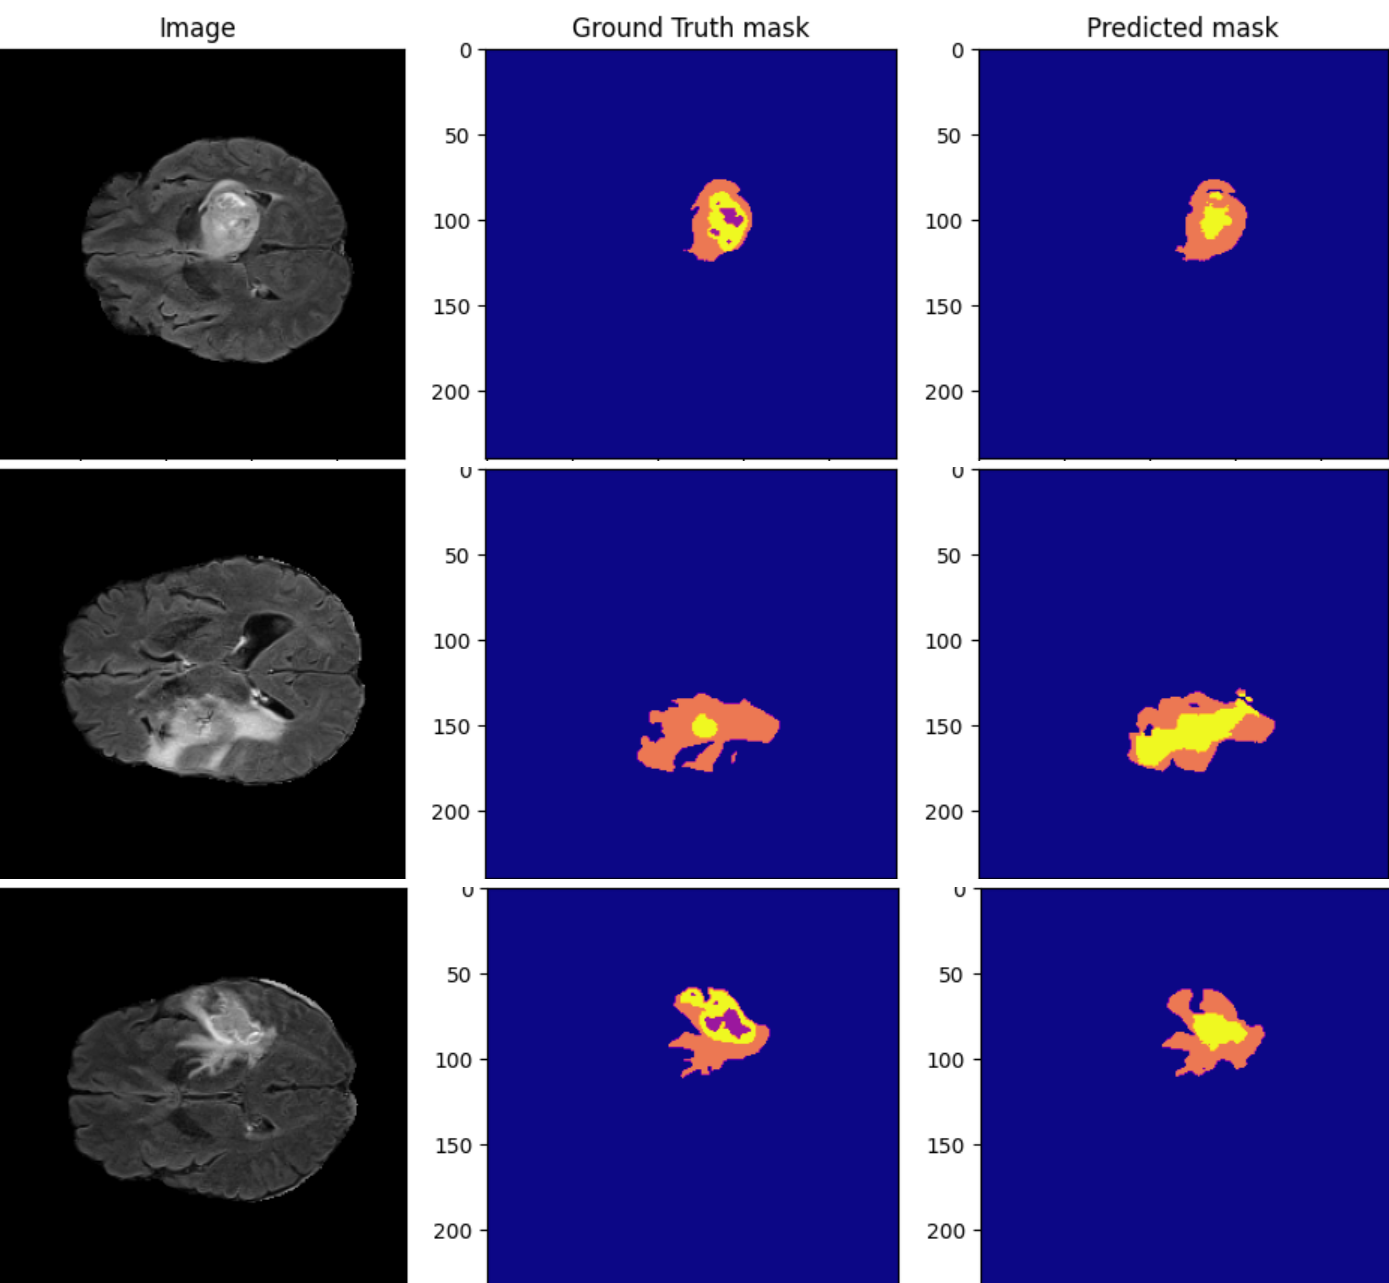
\includegraphics[height=4.2in]{Results/Chapter5Figs/mask_preds.png}
    \else
      \includegraphics[bb = 92 86 545 742, height=4.5in]{mask_pred}
    \fi
    \caption{Tumour mask predictions on test images. Column 1 shows the actual image, followed by the \textbf{Ground truth mask} and the \textbf{Model predictions}}
    \label{mask_pred}
  \end{center}
\end{figure}

The above picture shows some examples of ground-truth segmentation masks and the masks predicted by the UNet model.

\vspace{8mm}
\section{MTL joint segmentation-classification results}\label{MTL_results}
\vspace{3mm}
We experimented with 2 versions of the MTL model (as explained in section \ref{MTL}). One was with just the middle slice = 70 being used as the training set, and another where 10 slices were sampled across all the scans. To get the best possible extent of the nature of model discrimination, we performed the experiment with \textbf{T1-weighted} and \textbf{Flair} images separately. The results are summarized as: 

%3 tables: Flair middle-slice, T1 middle-slice, Flair 10 slices
\vspace{5mm}
\begin{table}[H]
\centering
\begin{tabular}{ c{2cm} c{2cm} c{2cm} c{2cm} c{2cm} }
 \hline
 \multicolumn{5}{c}{\thead{Middle slice : T1-weighted}} \\
 [0.8ex]
 \hline
  \thead{ $\lambda$} &\thead{Mean IoU} & \thead{AUC} & \thead{Accuracy} & \thead{Precision}\\  [0.8ex]
 \hline
  0.1  & 0.735 &0.526 &0.51 & 0.55     &  \\  [0.8ex]
 0.3  &  0.714 & 0.531 & 0.45 & 0.48 & \\  [0.8ex]
0.5  & 0.719 & 0.512 & 0.46 & 0.52  & \\  [0.8ex]
  0.7 & 0.702 & \cellcolor{yellow}\textbf{0.599} & 0.50 & 0.58 &  \\  [0.8ex]
   0.9 & 0.695 & 0.541 & 0.55 & 0.60\\  [0.8ex]

 \hline
\end{tabular}
\caption{Performance of 2D midddle slice MTL (T1)}
\label{table:1}
\end{table}
\vspace{3mm}
\begin{table}[H]
\centering
\begin{tabular}{ c{2cm} c{2cm} c{2cm} c{2cm} c{2cm}  }
 \hline
 \multicolumn{5}{c}{\thead{Middle slice : FLAIR}} \\
 [0.8ex]
 \hline
  \thead{ $\lambda$} & \thead{Mean IoU} & \thead{AUC} & \thead{Accuracy} & \thead{Precision}\\  [0.8ex]
 \hline
 0.1  &  0.868   & 0.542 & 0.58 & 0.58  \\  [0.8ex]
  0.3 & 0.845   & 0.587 & 0.53 & 0.60   \\  [0.8ex]
  0.5 & 0.858 &0.536 &0.52 &  0.56\\  [0.8ex]
  0.7 & 0.851 & 0.534 & 0.51  & 0.56\\  [0.8ex]
  0.9 & 0.793 & 0.441 & 0.45 & 0.50 \\

 \hline
\end{tabular}
\caption{Performance of 2D midddle slice MTL (Flair)}
\label{table:1}
\end{table}
\vspace{3mm}


\begin{table}[H]
\centering
\begin{tabular}{ c{2cm} c{2cm} c{2cm} c{2cm} c{2cm}   }
 \hline
 \multicolumn{5}{c}{\thead{10 sampled slice : Flair}} \\
 [0.8ex]
 \hline
  \thead{ $\lambda$} &\thead{Mean IoU} & \thead{AUC} & \thead{Accuracy} & \thead{Precision}\\  [0.8ex]
 \hline
 0.1 & \cellcolor{yellow}\textbf{0.898}  & 0.4712   & 0.46 & 0.47  \\  [0.8ex]
 0.3 & 0.890   & 0.516 & 0.53 & 0.52   \\  [0.8ex]
 0.5 &  0.882 & 0.497 & 0.51 & 0.50  \\  [0.8ex]
  0.7 & 0.846 & 0.548 & 0.56 & 0.53 \\  [0.8ex]

 \hline
\end{tabular}
\caption{Performance of 2D 10-slice MTL (Flair)}
\label{table:1}
\end{table}
\vspace{3mm}

As can be inferred, the highest AUC \textbf{0.599} is obtained for middle-slice MTL version for the \textbf{T1-weighted} images. The highest mean IoU score over 2 classes segmentation \textbf{0.898} is obtained for the \textbf{Flair} modality by sampling 10 slices. 

\section{Volumetric Projection results}\label{volumetric_results}
\vspace{3mm}
We experimented with 3 kinds of projections: \textbf{Mean, Maximum and Standard Deviation} projections (section \ref{volumetric}). The results of axis 1 (axial direction) for all 3 kinds of projections are depicted below:

\begin{table}[H]
\centering
\begin{tabular}{ c c c c }
 \hline
 \multicolumn{4}{c}{\thead{3 kinds of projection (axial)}} \\
 [0.8ex]
 \hline
  \thead{Projection} & \thead{AUC} & \thead{Accuracy} & \thead{Precision}\\  [0.8ex]
 \hline
 Maximum  & 0.5416  & 0.53 & 0.51  \\  [0.8ex]
 Standard Deviation &  0.5467   & 0.49 & 0.49    \\  [0.8ex]
 Mean &  0.5312 & 0.51 & 0.51   \\  [0.8ex]

 \hline
\end{tabular}
\caption{Projection Performance (axial direction)}
\label{table:1}
\end{table}
\vspace{3mm}

It was observed that the Standard Deviation projection was giving the best results, and so SD projections was tested along all 3 axes: axial, coronal and saggital.
\vspace{3mm}
\begin{table}[H]
\centering
\begin{tabular}{ c c c c }
 \hline
 \multicolumn{4}{c}{\thead{Standard Deviation Projection: 3 axes}} \\
 [0.8ex]
 \hline
  \thead{Axis} & \thead{AUC} & \thead{Accuracy} & \thead{Precision}\\  [0.8ex]
 \hline 
 AXIAL  & \cellcolor{yellow}\textbf{0.5884}    & 0.50 & 0.43 \\  [0.8ex]
 CORONAL &  0.4905  & 0.49 & 0.49   \\  [0.8ex]
 SAGGITAL & 0.5058 & 0.49 & 0.49 \\

 \hline
\end{tabular}
\caption{3 Axis Performance (SD projections)}
\label{table:1}
\end{table}
\vspace{3mm}
\textbf{EfficientNet B7} with \textbf{SD projection (along axial direction)} was the best performance with AUC of \textbf{0.5884}.





\section{Cascaded cropped-mask-results}\label{cropped_results}
\vspace{3mm}
In the cascaded cropped segmentation-classification model (section \ref{cropped_cascaded}), we experimented using 2 strategies: (a) With pre-determined slice number across train and test datasets (section \ref{2D_cropped}) (b) With 5-stack volume by finding the slice with best tumour visibility (section \ref{3D_cropped})
\vspace{3mm}

\textbf{EfficientNet B3, EfficientNet B7} and \textbf{ResNet32} were used for the pre-determined slice version with \textbf{slice = 70} used as the unanimous slice number. The performances are summarized below:
\vspace{3mm}

\begin{table}[H]
\centering
\begin{tabular}{ c c c c }
 \hline
 \multicolumn{4}{c}{\thead{2D slice cascaded model}} \\
 [0.8ex]
 \hline
  \thead{Model} & \thead{AUC} & \thead{Accuracy} & \thead{Precision}\\  [0.8ex]
 \hline
 EfficientNet B3  & 0.6250   & 0.47 & 0.47 \\  [0.8ex]
 EfficientNet B7 &  0.4783   & 0.47 & 0.48    \\  [0.8ex]
 ResNet34 &  \cellcolor{yellow}\textbf{0.6342} & \cellcolor{yellow}\textbf{0.57} & \cellcolor{yellow}\textbf{0.53}  \vspace{3mm}\\ 
 \hline
\end{tabular}
\caption{Results of 2D cascaded model}
\label{table:1}
\end{table}
\vspace{3mm}


We proceeded to the 3D 5-slice stacked volume version of the cascaded model, and the classifiers were changed as: \textbf{EfficientNet B0, EfficientNet B3, EfficientNet B7, ResNet18} and \textbf{ResNet34}. 5 fold cross-validation was utilized with \textbf{Stratified K-folds} strategy to keep the class label ratio similar along all the fold partitions. Henceforth, we used \textbf{5-fold-cross-validation} for each phase. The data mentioned in the tables mention the average AUC/Accuracy with the Standard Deviation obtained across all 5 folds.

\begin{table}[H]
\centering
\begin{tabular}{ c c c c}
 \hline
 \multicolumn{4}{c}{\thead{5-slice 3D cascaded (single classifier)}} \\
 [0.8ex]
 \hline
  \thead{Axis} & \thead{model} & \thead{AUC} & \thead{Accuracy}\\  [0.8ex]
 \hline
 \multirow{5}{4em}{AXIAL}& EffNet B0 & $0.532 \pm 0.038$  & $0.522 \pm 0.046$ & \vspace{3mm}
&EffNet B3 & $0.4942 \pm 0.034$ & $0.506 \pm 0.021$  & \vspace{3mm} 
&EffNet B7 & $0.4455 \pm 0.058$ & $0.5099 \pm 0.017$ & \vspace{3mm}
&ResNet18 & $0.553 \pm 0.062$ & $0.510 \pm 0.047$  & \vspace{3mm}
&ResNet34 & \cellcolor{yellow}\boldmath{$0.641 \pm 0.187$ } & \cellcolor{yellow}\boldmath{$0.620 \pm 0.150$} & 
\hline
\multirow{5}{4em}{CORONAL}& EffNet B0 & $0.546 \pm 0.052$ & $0.493 \pm 0.019$ & \vspace{3mm}
&EffNet B3 & $0.521 \pm 0.044$ & $0.513 \pm 0.018$ & \vspace{3mm} 
&EffNet B7 & $0.475 \pm 0.055$ & $0.511 \pm 0.017$  & \vspace{3mm}
&ResNet18 & $0.640 \pm 0.190$ & $0.608 \pm 0.182$ & \vspace{3mm}
&ResNet34 & $0.586 \pm 0.121$ & $0.574 \pm 0.090$ & 
\hline
\multirow{5}{4em}{SAGGITAL}& EffNet B0 & $0.490 \pm 0.086$ & $0.511 \pm 0.018$ & \vspace{3mm}
&EffNet B3 & $0.505 \pm 0.054 $ & $0.511 \pm 0.017$  & \vspace{3mm} 
&EffNet B7 & $0.509 \pm 0.060$ & $0.488 \pm 0.017$ & \vspace{3mm}
&ResNet18 & $0.582 \pm 0.147$ & $0.576 \pm 0.118$ & \vspace{3mm}
&ResNet34 &  $0.575 \pm 0.183$& $0.551 \pm 0.150$ & 
 \hline
\end{tabular}
\caption{Results of 5-slice 3D cascaded (single model)}
\label{table:1}
\end{table}
\vspace{3mm}

The highest AUC of \boldmath{$0.641 \pm 0.187$} is obtained for \textbf{ResNet34} in the \textbf{axial direction} (as highlighted in the tables). Various kinds of ensembles were also tested with, and in majority of the cases they gave better performances.
\vspace{5mm}
\begin{table}[H]
\centering
\begin{tabular}{ c c c c}
 \hline
 \multicolumn{4}{c}{\thead{5-slice 3D cascaded (ensemble)}} \\
 [0.8ex]
 \hline
  \thead{Axis} & \thead{model} & \thead{AUC} & \thead{Accuracy}\\  [0.8ex]
 \hline
 \multirow{3}{4em}{AXIAL}& ResNet18 + ResNet34 & \cellcolor{yellow}\boldmath{$0.736 \pm 0.160$} & \cellcolor{yellow}\boldmath{$ 0.662 \pm 0.148$} & \vspace{3mm}
&ResNet18 + EffNet B3 & $0.692 \pm 0.169$  & $0.653 \pm 0.140$ & \vspace{3mm} 
&ResNet34 + EffNet B3 & $0.713 \pm 0.160$ & $0.662 \pm 0.148$ & 
\hline
\multirow{3}{4em}{CORONAL}& ResNet18 + ResNet34 & \cellcolor{yellow}\boldmath{$0.721 \pm 0.174$} & \cellcolor{yellow}\boldmath{$ 0.693 \pm 0.140$} & \vspace{3mm}
&ResNet18 + EffNet B3 & $0.680 \pm 0.199$ & $0.637 \pm 0.172$ & \vspace{3mm} 
&ResNet34 + EffNet B3 & $0.637 \pm 0.177$ & $0.608 \pm 0.136$ & 
\hline
\multirow{3}{4em}{SAGGITAL}& ResNet18 + ResNet34 & $0.707 \pm 0.202$ & $0.684 \pm 0.154$ & \vspace{3mm}
&ResNet18 + EffNet B3 & $0.629 \pm 0.189$ & $0.609 \pm 0.135$ & \vspace{3mm} 
&ResNet34 + EffNet B3 & $0.715 \pm 0.146$ & $0.671 \pm 0.104$ & 
 \hline
\end{tabular}
\caption{Results of 5-slice 3D cascaded (ENSEMBLE)}
\label{table:1}
\end{table}
\vspace{3mm}
For ensembles, the highest AUC \boldmath{$0.736 \pm 0.160$} is obtained for the \textbf{ResNet18 and ResNet34 ensemble} in the \textbf{axial direction} and the highest Accuracy \bolmath{$0.693 \pm 0.140$} is obtained for the same emsemble in the \textbf{coronal direction} (as highlighted in the tables).


\section{3-axis Ensemble Results}\label{3_axis_results}
\vspace{3mm}
The 3-axis-ensemble (section \ref{3-axis-ensemble}) uses the same MRI scan to sample slices across 3 different axis directions, and then trains separte UNet and classifiers for each direction.
\vspace{4mm}

\begin{table}[H]
\centering
\begin{tabular}{ c c c c}
 \hline
 \multicolumn{3}{c}{\thead{3-axis ensemble}} \\
 [0.8ex]
 \hline
  \thead{Model} & \thead{AUC} & \thead{Accuracy} \\  [0.8ex]
 \hline
 ResNet18  &  $0.711 \pm 0.198$   & $0.665 \pm 0.171$  \\  [0.8ex]
 ResNet34 &  \cellcolor{yellow}\boldmath{$0.721 \pm 0.231$}  & \cellcolor{yellow}\boldmath{$0.700 \pm 0.205$ }  & \vspace{3mm}\\ 
 \hline
\end{tabular}
\caption{Results of 3-axis Ensemble}
\label{table:1}
\end{table}
\vspace{3mm}


As a conclusion across all models tested, we were able to attain the highest AUC \textbf{0.736} in \textbf{ResNet18 + ResNet34 ensemble} in the axial directional case. This surpasses the current Kaggle leaderboard AUC of abc.

\vspace{5mm}
AUC in the experimentation refers to Area under curve, which has been explained in Appendix A (\ref{AUC}). AUC is calculated as the Area Under the $Sensitivity$(TPR)-$(1-Specificity)$(FPR) Curve. True Positive refers to the samples which were classified as '1' (methylated) and it was a correct classification, while FP refers to a '1' classification which was False (truth was unmethylated).
\\
\begin{center}
    $Accuracy$ = $\displaystyle\frac{TP+TN}{TP+TN+FP+FN}$
\\\vspace{2mm}
$Precision $= $\displaystyle\frac{TP}{TP+FP}$
\\\vspace{2mm}
$Recall $=$ \displaystyle\frac{TP}{TP+FN}$
\\\vspace{4mm}
\end{center}





% \cite{texbook}

% \subsection{sub first paragraph}
% ... and some more ...



% above code has been macro-fied in Classes/MacroFile.tex file
%\InsertFig{\IncludeGraphicsH{aflow}{6in}{92 86 545 742}}{Airfoil Picture}{FigAir}

% So as we have now labelled it we can reference it, like so (\ref{FigKaggleLeaderboard}) and it
% is on Page \pageref{FigKaggleLeaderboard}. And as we can see, it is a very nice picture and we
% can talk about it all we want and when we are tired we can move on to the next
% chapter ...

\ifpdf
  \pdfbookmark[2]{bookmark text is here}{And this is what I want bookmarked}
\fi
% ------------------------------------------------------------------------


%%% Local Variables: 
%%% mode: latex
%%% TeX-master: "../thesis"
%%% End: 
